\section{Два примера $d^2\sigma/dxdQ^2$}
\label{sec:examples_extrapolated_region}
\begin{figure}[!h]
\centering
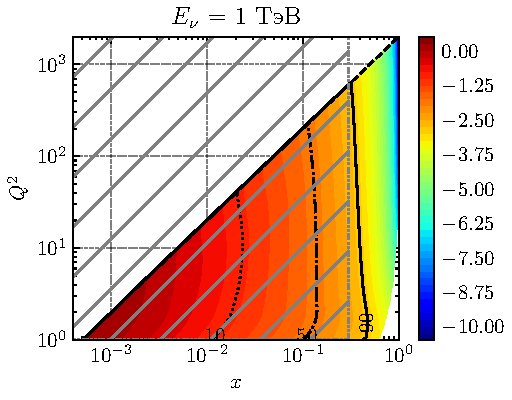
\includegraphics[width=0.97\linewidth]{images/NuProp/cdfxq2_cc_proton_CT18ZNNLO_14_1000.pdf}
\caption{Зависимость кумулятивного нормированного сечения $F_{\sigma}(x,Q^2)$ в зависимости от переменной Бъеркена $x$ и переменной $Q^2$ для энергии нейтрино $E_{\nu} = 1$ TeV для модели партонных распределений CTEQ15\cite{ncteq15}. }
\label{Pp3}
\end{figure}
\begin{figure}[!h]
\centering
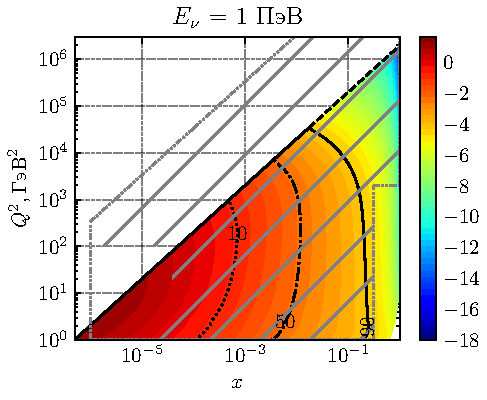
\includegraphics[width=0.97\linewidth]{images/NuProp/cdfxq2_cc_proton_CT18ZNNLO_14_1000000.pdf}
\caption{Зависимость кумулятивного нормированного сечения $F_{\sigma}(x,Q^2)$ в зависимости от переменной Бъеркена $x$ и переменной $Q^2$ для энергии нейтрино $E_{\nu} = 1$ PeV для модели партонных распределений CTEQ15\cite{ncteq15}.}
\label{Pp6}
\end{figure}
